% streaming_pipeline_intro.tex
\documentclass[aspectratio=169,11pt]{beamer}

\usetheme{Madrid}
\usecolortheme{default}
\usefonttheme{professionalfonts}

% Packages
\usepackage[utf8]{inputenc}
\usepackage[T1]{fontenc}
\usepackage{lmodern}
\usepackage{amsmath, amssymb}
\usepackage{booktabs}
\usepackage{graphicx}
\usepackage{tikz}
\usetikzlibrary{arrows.meta, positioning, shapes, calc, fit}
\usepackage{listings}
\usepackage{xspace}
\usepackage{hyperref}

% Pseudocode language (tool- and language-agnostic)
\lstdefinelanguage{PseudoStream}{
  morekeywords={source,sink,filter,map,flatmap,window,aggregate,join,withKey,sideOutput,
  watermark,assignTimestamp,trigger,allowedLateness,state,checkpoint,exactlyOnce,atLeastOnce,
  keyBy,process,onTimer,session,tumbling,hopping,reduce,union,branch},
  sensitive=true,
  morecomment=[l]{//},
  morecomment=[s]{/*}{*/},
  morestring=[b]"
}
\lstset{
  language=PseudoStream,
  basicstyle=\ttfamily\small,
  keywordstyle=\bfseries,
  commentstyle=\itshape,
  showstringspaces=false,
  frame=single,
  columns=fullflexible,
  keepspaces=true,
  tabsize=2,
  escapeinside={(*}{*)},
  breaklines=true,
  breakatwhitespace=true
}

\newcommand{\term}[1]{\textbf{#1}}
\newcommand{\mins}[1]{\textit{(#1 min)}}

\setbeameroption{hide notes}
% \setbeameroption{show notes on second screen=right}

\title{Streaming \& Pipeline Processing}
\subtitle{Event Time, Windows, State, and Reliable Delivery}
\author{Diogo Ribeiro}
\date{\today}

\begin{document}

% ------------------------------------------------------------------
\begin{frame}
  \titlepage
  \note{Emphasize neutrality: concepts apply across engines, brokers, and storage systems.}
\end{frame}

% ------------------------------------------------------------------
\begin{frame}{Learning Objectives}
  By the end, participants can:
  \begin{itemize}
    \item Explain event time vs processing time and watermarks.
    \item Choose windowing strategies and triggers for different problems.
    \item Design stateful operators and manage late/duplicate data.
    \item Reason about delivery guarantees and end-to-end exactly-once.
    \item Join streams and handle backpressure safely.
    \item Test, observe, and operate streaming pipelines in production.
  \end{itemize}
\end{frame}

% ------------------------------------------------------------------
\begin{frame}{Agenda \mins{5}}
  \begin{enumerate}
    \item Why Streaming? \mins{10}
    \item Time Model: Event vs Processing Time \& Watermarks \mins{15}
    \item Windows, Triggers, Lateness \mins{20}
    \item Stateful Processing \& Delivery Guarantees \mins{20}
    \item Joins, Backpressure, Fault Tolerance \mins{15}
    \item Testing, Observability, Cost \mins{10}
    \item Exercises \& Wrap-up \mins{10}
  \end{enumerate}
\end{frame}

% =========================
\section{Why Streaming?}
% =========================
\begin{frame}{Motivation \mins{10}}
  \begin{itemize}
    \item Many domains are \term{event-driven}: telemetry, payments, logs, sensors.
    \item Streaming yields \term{low latency} insights and reactive products.
    \item Unified batch+stream architectures reduce duplication and staleness.
    \item Cost/ops trade-offs: continuous compute vs scheduled batch.
  \end{itemize}
  \note{Position streaming as a spectrum: micro-batch $\rightarrow$ true streaming.}
\end{frame}

% =========================
\section{Time, Watermarks}
% =========================
\begin{frame}{Event Time vs Processing Time \mins{8}}
  \begin{itemize}
    \item \term{Event Time}: when an event actually happened.
    \item \term{Processing Time}: when the system observed it.
    \item Networks, buffers, and clocks cause reordering and delay.
  \end{itemize}
\end{frame}

\begin{frame}{Watermarks \mins{7}}
  \begin{itemize}
    \item A \term{watermark} asserts that most events older than $T$ have arrived.
    \item Drives window completeness and trigger firing.
    \item Heuristics: fixed lag (e.g., eventTime - 2 min), source-derived, or adaptive.
  \end{itemize}
\end{frame}

\begin{frame}[fragile]{Timestamp Assignment \mins{5}}
\begin{lstlisting}
source("clicks")
  .assignTimestamp(event.ts)     // choose event time field
  .watermark(event.ts - 120s)    // simple fixed-lag watermark
  .map(...)
  .sink("analytics")
\end{lstlisting}
\note{Avoid engine specifics; the idea is: pick a timestamp and a watermark policy.}
\end{frame}

% =========================
\section{Windows, Triggers, Lateness}
% =========================
\begin{frame}{Windowing Strategies \mins{8}}
  \begin{itemize}
    \item \term{Tumbling}: fixed, non-overlapping ($[0,1),[1,2)$).
    \item \term{Hopping/Sliding}: fixed, overlapping (size, slide).
    \item \term{Session}: data-driven gaps, per key.
    \item \term{Global}: unbounded with triggers (e.g., count-based).
  \end{itemize}
\end{frame}

\begin{frame}{Triggers \& Accumulation \mins{7}}
  \begin{itemize}
    \item \term{Triggers}: when to emit (on watermark, processing time, count, custom).
    \item \term{Accumulation}: discard, accumulate, or accumulate+retract.
    \item Re-emit updates as late data refines results.
  \end{itemize}
\end{frame}

\begin{frame}{Late Data Handling \mins{5}}
  \begin{itemize}
    \item \term{Allowed Lateness}: accept events arriving after watermark by $\Delta$.
    \item Side outputs for too-late events (dead-letter, audit, or reprocess).
    \item Deduplication keys mitigate duplicates on retries.
  \end{itemize}
\end{frame}

\begin{frame}[fragile]{Windowed Aggregation (Pseudocode) \mins{6}}
\begin{lstlisting}
source("purchases")
  .assignTimestamp(event.ts)
  .watermark(event.ts - 2m)
  .keyBy(userId)
  .window(tumbling, size=5m)
  .aggregate(sum(amount))
  .trigger(onWatermark)
  .allowedLateness(1m)
  .sideOutput("late")
  .sink("user_spend_5m")
\end{lstlisting}
\end{frame}

% =========================
\section{State, Guarantees}
% =========================
\begin{frame}{Stateful Processing \mins{8}}
  \begin{itemize}
    \item Operator state: per-key or global.
    \item Timers: register callbacks for event/processing time.
    \item Snapshots/checkpoints persist state for recovery and exactly-once.
  \end{itemize}
\end{frame}

\begin{frame}[fragile]{Per-Key State Example \mins{6}}
\begin{lstlisting}
// Rolling unique URLs per user with TTL
source("clicks")
  .assignTimestamp(ts).watermark(ts - 1m)
  .keyBy(userId)
  .process(state.set("urls", TTL=24h)) { e =>
    state.urls.add(e.url)
    emit(size=state.urls.count(), userId=e.userId)
  }
  .sink("unique_urls")
\end{lstlisting}
\end{frame}

\begin{frame}{Delivery Semantics \mins{6}}
  \begin{itemize}
    \item \term{At-most-once}: may drop data, no duplicates.
    \item \term{At-least-once}: no data loss, duplicates possible.
    \item \term{Exactly-once} (effectively-once): no loss, no duplicates (with idempotence/transactions).
  \end{itemize}
  \note{End-to-end requires aligned semantics in source, processor, and sink.}
\end{frame}

\begin{frame}{Exactly-Once Pattern \mins{6}}
\begin{itemize}
  \item Input: partition+offset or sequence IDs.
  \item Processing: transactional state snapshots (barriers/checkpoints).
  \item Output: idempotent/transactional sink with commit on checkpoint.
\end{itemize}
\end{frame}

% =========================
\section{Joins, Backpressure, Faults}
% =========================
\begin{frame}{Stream–Stream Joins \mins{8}}
  \begin{itemize}
    \item Requires windows + time alignment + per-key state.
    \item \term{Inner/Left/Right/Outer} joins over temporal intervals.
    \item Reordering late events: update/retract results as needed.
  \end{itemize}
\end{frame}

\begin{frame}[fragile]{Join Sketch (Pseudocode) \mins{6}}
\begin{lstlisting}
source("orders").assignTimestamp(ts)
  .join(source("payments").assignTimestamp(ts))
  .onKey(orderId)
  .within(window=15m)           // temporal join bound
  .trigger(onWatermark)
  .emit(orderId, status)
  .sink("order_payment_join")
\end{lstlisting}
\end{frame}

\begin{frame}{Backpressure \& Flow Control \mins{7}}
  \begin{itemize}
    \item When downstream is slower than upstream, buffers fill.
    \item Strategies: bounded queues, rate limiting, adaptive batching.
    \item Scale-out hotspots by key partitioning and rebalancing.
  \end{itemize}
\end{frame}

\begin{frame}{Fault Tolerance \mins{8}}
  \begin{itemize}
    \item Checkpoints + replay from durable logs.
    \item Exactly-once sinks: two-phase commit or idempotent upserts.
    \item Stateless vs stateful recovery times and trade-offs.
  \end{itemize}
\end{frame}

% =========================
\section{Testing, Observability, Cost}
% =========================
\begin{frame}{Testing Strategies \mins{6}}
  \begin{itemize}
    \item Deterministic test harnesses: feed records with timestamps.
    \item Golden files for windowed outputs under reordering/latency.
    \item Property-based tests: idempotence, associativity of combiners.
  \end{itemize}
\end{frame}

\begin{frame}{Observability \mins{4}}
  \begin{itemize}
    \item Metrics: input/output rates, watermark lag, busy time, backlogs.
    \item Logs and event samples for debugging late/duplicate paths.
    \item Traces across source $\rightarrow$ processor $\rightarrow$ sink.
  \end{itemize}
\end{frame}

\begin{frame}{Cost \& Capacity \mins{4}}
  \begin{itemize}
    \item Cardinality drives state size; state drives memory and checkpoint cost.
    \item Window width and lateness increase storage and compute.
    \item Right-size partitions and autoscaling policies.
  \end{itemize}
\end{frame}

% =========================
\section{Exercises}
% =========================
\begin{frame}{Exercise 1: Window Choices \mins{6}}
  \textbf{Scenario:} Rolling user activity dashboard.\\
  \textbf{Task:} Pick window type (tumbling/hopping/session) and trigger policy.\\
  \textbf{Deliverable:} One-slide justification (latency vs accuracy vs cost).
\end{frame}

\begin{frame}{Exercise 2: Late Data Plan \mins{6}}
  \textbf{Scenario:} Mobile telemetry with flaky connectivity.\\
  \textbf{Task:} Choose watermark, allowed lateness, and side-output policy.\\
  \textbf{Deliverable:} Policy doc: how to reconcile late updates in downstream stores.
\end{frame}

\begin{frame}{Exercise 3: Exactly-Once Sketch \mins{6}}
  \textbf{Scenario:} Deduct credits once per order.\\
  \textbf{Task:} Outline idempotent keys, checkpoint cadence, and sink commit flow.\\
  \textbf{Deliverable:} Sequence diagram with failure/retry paths.
\end{frame}

% =========================
\section{Design Patterns}
% =========================
\begin{frame}{Reusable Patterns \mins{8}}
  \begin{itemize}
    \item \term{Dead Letter Stream}: quarantine malformed or too-late events.
    \item \term{Outbox/Inbox}: transactional handoff between services.
    \item \term{Upsert Sink}: idempotent writes keyed by natural/business IDs.
    \item \term{Rekey/Compaction}: change partitioning without data loss.
    \item \term{Side Outputs}: route anomalies without blocking main flow.
  \end{itemize}
\end{frame}

% =========================
\section{Visual Model}
% =========================
\begin{frame}{Reference Architecture (Conceptual) \mins{6}}
\centering
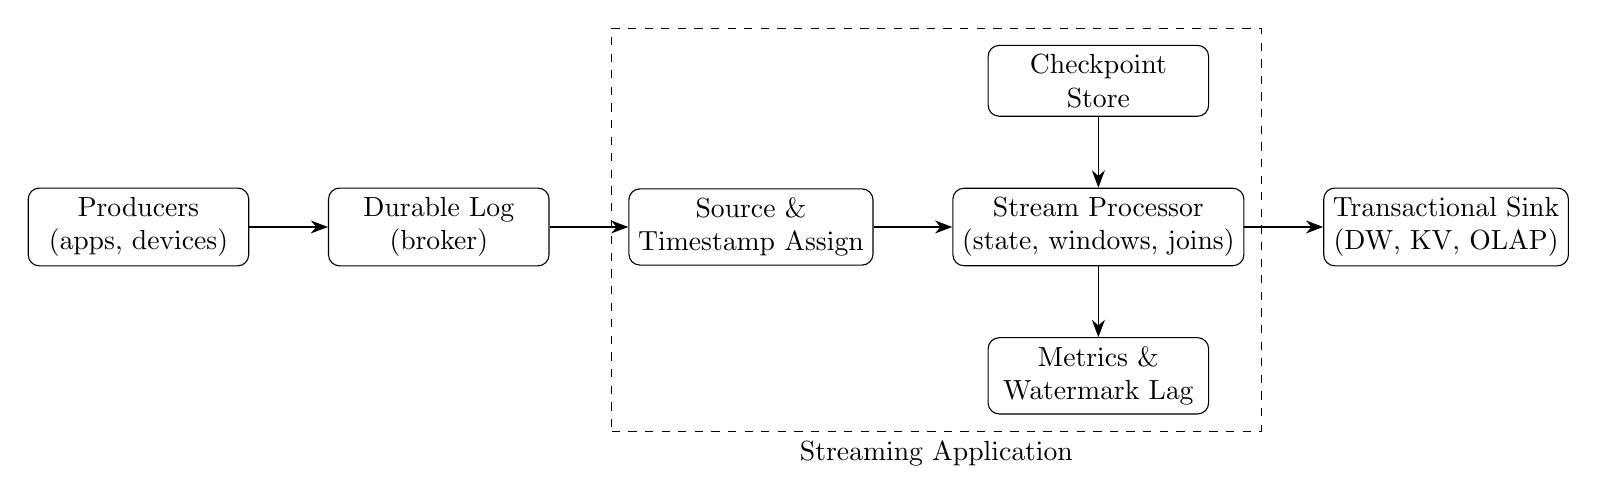
\begin{tikzpicture}[
  box/.style={rectangle, rounded corners, draw, minimum width=2.8cm, minimum height=0.9cm, align=center},
  >={Stealth[length=2.2mm]},
  node distance=0.9cm and 1.0cm
]
\node[box] (producers) {Producers\\(apps, devices)};
\node[box, right=of producers] (broker) {Durable Log\\(broker)};
\node[box, right=of broker] (ingest) {Source \&\\Timestamp Assign};
\node[box, right=of ingest] (proc) {Stream Processor\\(state, windows, joins)};
\node[box, right=of proc] (sink) {Transactional Sink\\(DW, KV, OLAP)};
\node[box, below=of proc] (obs) {Metrics \&\\Watermark Lag};
\node[box, above=of proc] (ckpt) {Checkpoint\\Store};

\draw[->] (producers) -- (broker);
\draw[->] (broker) -- (ingest);
\draw[->] (ingest) -- (proc);
\draw[->] (proc) -- (sink);
\draw[->] (proc) -- (obs);
\draw[->] (ckpt) -- (proc);

\node[draw, dashed, fit=(ingest) (proc) (ckpt) (obs), inner sep=6pt, label=below:Streaming Application] {};
\end{tikzpicture}
\note{Highlight separation of concerns: ingestion, processing, state/checkpoints, outputs.}
\end{frame}

% =========================
\section{Wrap-up}
% =========================
\begin{frame}{Quick Quiz \mins{6}}
  \begin{enumerate}
    \item Why prefer event time over processing time for aggregation?
    \item What role do watermarks play?
    \item Compare tumbling, hopping, and session windows.
    \item What is end-to-end exactly-once and how is it achieved?
  \end{enumerate}
\end{frame}

\begin{frame}{Key Takeaways \mins{3}}
  \begin{itemize}
    \item Treat time as data; design with watermarks and late events in mind.
    \item Windows + triggers define latency vs accuracy trade-offs.
    \item State and checkpoints enable correctness under failures.
    \item Backpressure and idempotence are operational essentials.
  \end{itemize}
\end{frame}

% =========================
\appendix
% =========================
\begin{frame}{Appendix: Glossary}
\small
\begin{tabular}{@{}ll@{}}
\toprule
Term & Meaning \\
\midrule
Event Time & Timestamp of occurrence \\
Processing Time & Timestamp of observation \\
Watermark & Lower bound on unseen event time \\
Window & Temporal slice for grouping \\
Trigger & Rule for emitting results \\
Allowed Lateness & Grace period for late events \\
State & Persistent operator memory \\
Checkpoint & Consistent snapshot for recovery \\
Backpressure & Slower downstream throttles upstream \\
\bottomrule
\end{tabular}
\end{frame}

\begin{frame}{Appendix: Timing Plan (90–120 min)}
\small
\begin{tabular}{@{}ll@{}}
\toprule
Segment & Minutes \\
\midrule
Why Streaming & 10 \\
Time \& Watermarks & 15 \\
Windows \& Triggers & 20 \\
State \& Guarantees & 20 \\
Joins \& Backpressure & 15 \\
Testing/Observability/Cost & 10 \\
Exercises (3) & 18 \\
Quiz/Wrap & 7 \\
Buffer / Q\&A & 5--15 \\
\bottomrule
\end{tabular}
\end{frame}

\begin{frame}[plain]
  \centering
  \Huge Thank you!
\end{frame}

\end{document}
